\begin{figure*}[t]
  \centering
  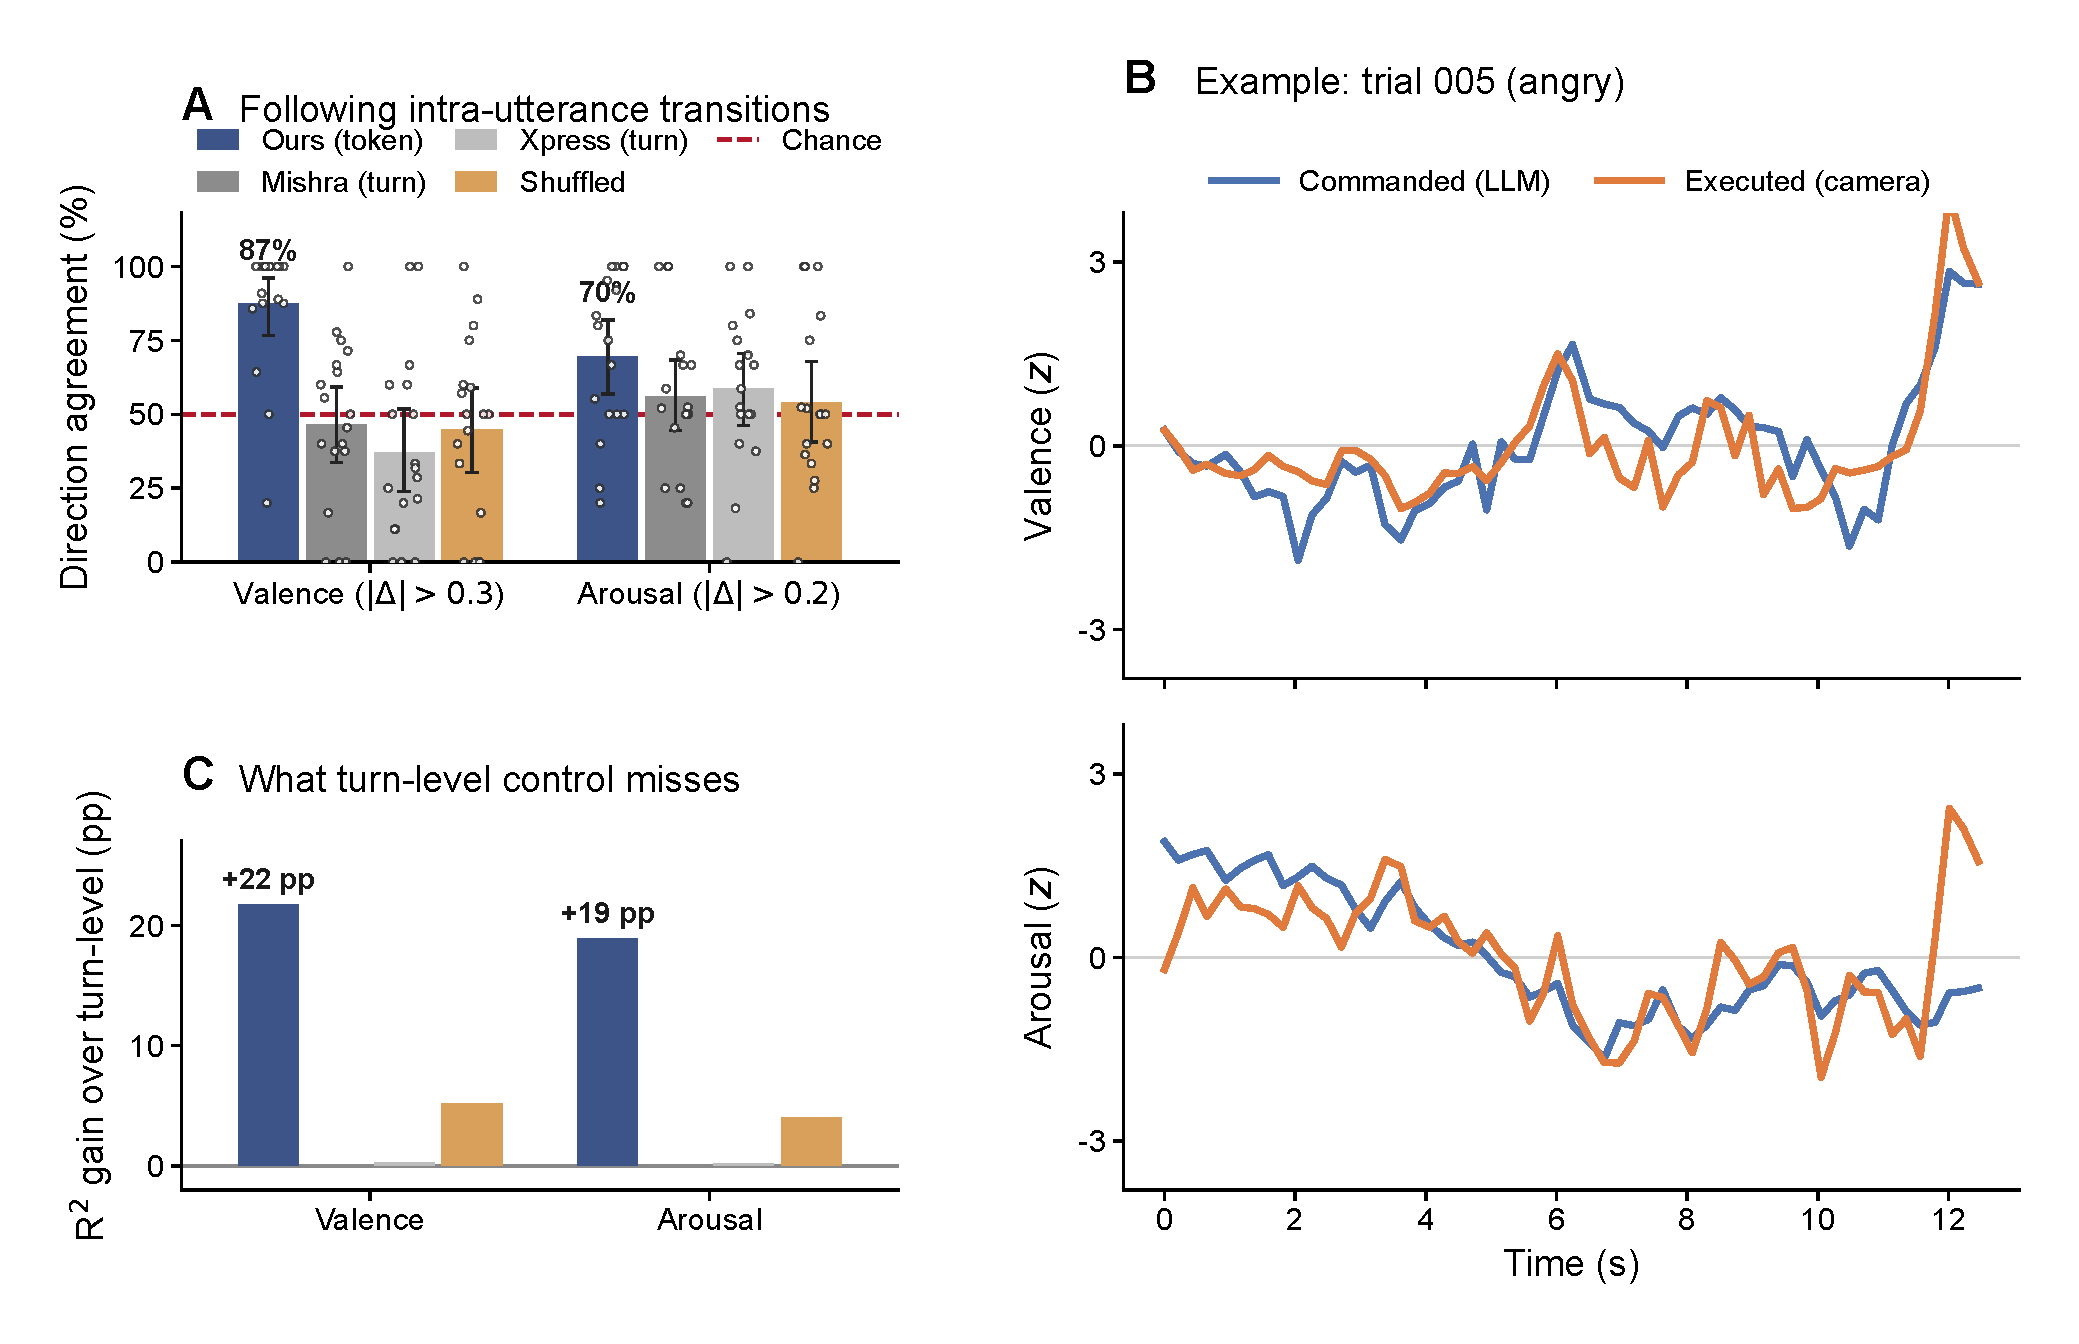
\includegraphics[width=\textwidth]{experiment/C/C1/output/multicond_noanchor_20260731/paper/c1_main_figure.pdf}
  \caption{Closed-loop execution of token-level affect under a four-condition, same-session comparison ($n{=}20$ utterances).
  \textbf{(A)}~Direction agreement between commanded affect transitions (2\,s window) and camera readback: ours reaches 87\% (valence, 95\% CI [77, 96]) and 70\% (arousal), while turn-level (Mishra, Xpress) and time-shuffled baselines stay at chance (dashed line).
  Bars: trial-mean accuracy with trial-clustered bootstrap 95\% CIs; dots: per-trial accuracy.
  \textbf{(B)}~Representative trial 005: fixed-lag-aligned, $z$-scored commanded (LLM) versus executed (camera) trajectories.
  \textbf{(C)}~Facial variance explained beyond a turn-level constant expression: token-level control adds +22/+19\,pp (valence/arousal); baselines add none by construction.
  All conditions share one fixed execution+detection lag (0.5\,s); FER readback is linearly calibrated on the static-face conditions.}
  \label{fig:c1_main}
\end{figure*}
